\documentclass[spanish, a4paper, nobib]{tufte-handout}

% encoding
\usepackage[utf8]{inputenc}
\usepackage[T1]{fontenc}
\usepackage{lmodern}
\usepackage{babel}
\usepackage{pdfpages}

\frenchspacing
\usepackage[style=spanish]{csquotes}
\MakeAutoQuote{«}{»}

\usepackage{booktabs}
\usepackage{circuitikz}
\usepackage{siunitx}
\usepackage{amsmath}
\usepackage{nicefrac}

\graphicspath{
    {fotos/}
}

% hyperlink setup / metadata
\usepackage{hyperref}
\AfterPreamble{\hypersetup{
  %%pdfauthor={},
  %%pdftitle={},
  %%pdfsubject={},
}}

% document metadata
\author{Víctor Méndez}
\title{ONELE: Práctica 1}
\date{7-3-2024}

\begin{document}

\maketitle

\newthought{1. Ancho del spot principal difractado por una apertura}

«Se trata de obtener la semi-anchura del lóbulo principal de la radiación que emerge de la apertura en función del ancho de la apertura, para una longitud de onda fijada, y con un campo inicial uniforme.»

\begin{figure}[h]
    \begin{center}
        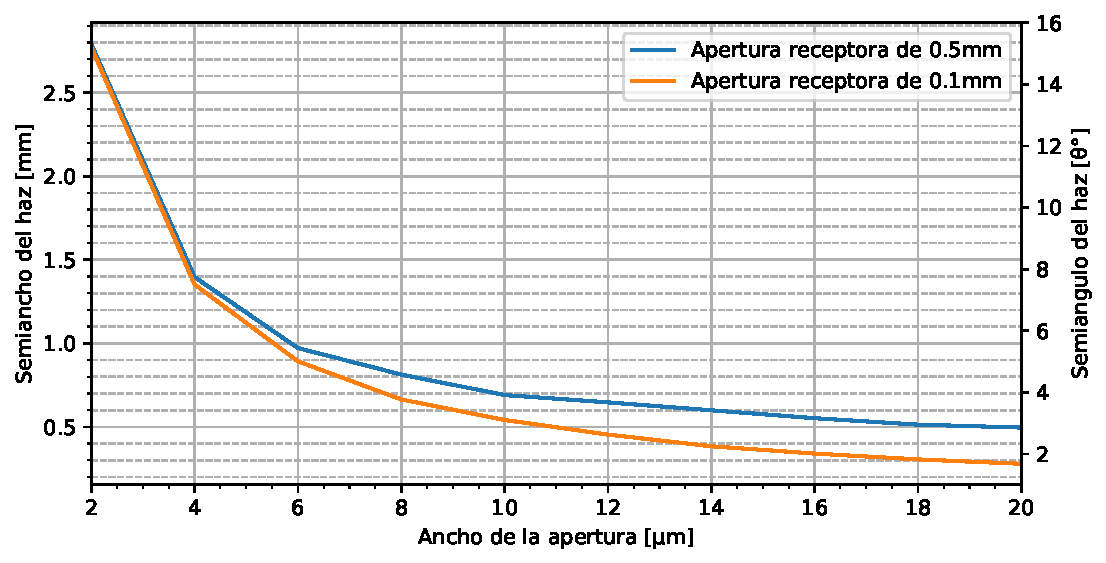
\includegraphics[width=300px]{p1.pdf}
    \end{center}
    \caption{Semiancho del haz en función de la apertura}
    \label{fig:p1}
\end{figure}

Las medidas descienden según $\sim\frac{1}{L}$; cuanto más grande la apertura menos se difracta la onda. Cuanto más baja la apertura receptora, más fiel es la medida al cálculo teórico que se haría aplicando la aproximación de Fraunhofer.

Con $z_{max}=\qty{10}{\milli\meter}$ podemos aplicar la aproximación de Fraunhofer, puesto que se cumple $\frac{L}{\lambda}\ll\frac{z}{L}$. En esta aproximación, con una apertura simple y un campo uniforme, el semi-ángulo del lóbulo principal viene dado por $\theta=\arcsin{\frac{\lambda}{L}}$, para $\frac{\lambda}{L}\simeq 0$ se puede aproximar por $\theta\simeq\frac{\lambda}{L}$. Finalmente, el semi-ancho viene dado por la tangente del ángulo\sidenote{Realmente, $\theta$ es tan pequeña que $\tan{\theta}\simeq\theta$. Con esta aproximación podemos decir que $\alpha\sim\theta$, justificando así la primera observación.}, $\alpha_{\nicefrac{1}{2}}=\tan{\theta}\cdot z_{max}$.

\newthought{2. Determinación de la anchura de una apertura}

«En el laboratorio se ha medido la anchura del spot principal que emerge de un pinhole y de una ranura utilizando un láser. Con esos datos y la ayuda de la gráfica del ejercicio anterior determine las anchuras estimadas de aquellos elementos.»

Si llamamos $\theta$ al semi-ángulo, $\alpha$ al ancho y aplicamos las equaciones de la aproximación nos queda lo siguiente.

\begin{align}
    \left.
        \begin{aligned}
            \theta &= \arcsin{\frac{\lambda}{L}}\quad \\
            \alpha &= 2 z \cdot \tan{\theta}
        \end{aligned}
    \right\} \Rightarrow L = \frac{\lambda}{\sin{\left(\arctan{\frac{\alpha}{2 z}}\right)}}
\end{align}

En el laboratorio medimos un ancho de \qty{53}{\milli\meter} y una distancia de \qty{320}{\milli\meter}. La apertura es entonces \qty{6.45}{\micro\meter}.

\newpage

\newthought{3. Radiación producida por una apertura múltiple de tipo grating}

«Se trata de visualizar el ángulo con que emerge una onda plana de un tipo particular de red de difracción. Se hallará el ángulo con que sale el lóbulo principal en función del ancho de la apertura.»

\begin{figure}[h]
    \begin{center}
        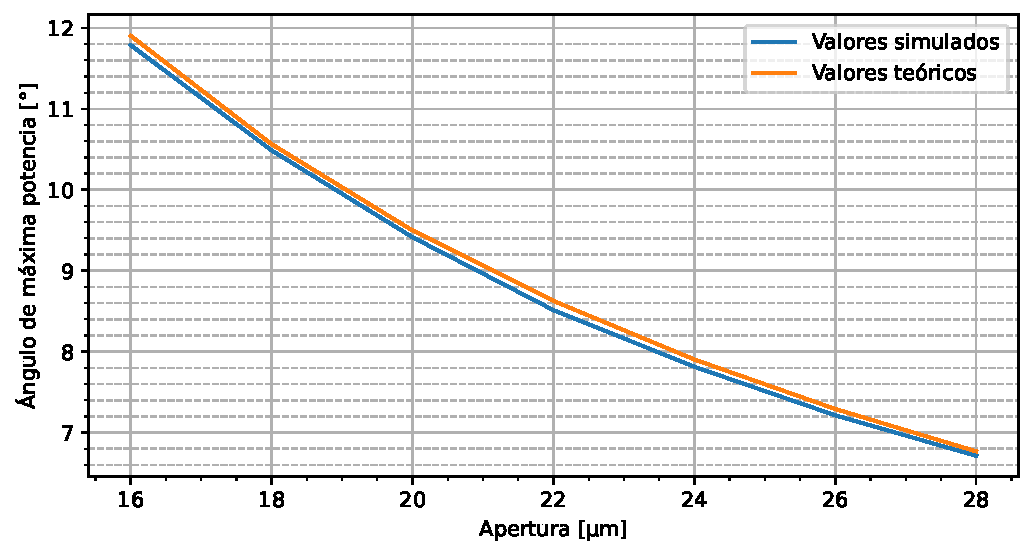
\includegraphics[width=300px]{p3.pdf}
    \end{center}
    \caption{Ángulo de potencia máxima en función de la apertura}
    \label{fig:p3}
\end{figure}

Si aproximamos la apertura con un coseno enventanado y aplicamos Fraunhofer nos queda

\begin{align}
    \vec{E}(x,\,y) &= E_0\cdot\Pi\left(\frac{x}{L}\right)\cos{(k_0 x)} \cdot \hat{z} \\
    \vec{E_k}(k_x,\,k_y) &= E_0\frac{L}{2}\cdot sinc\left(L(k_x \pm k_0)\right) \cdot \hat{z} \\
    \vec{E}(\theta ,\, r) &= j\frac{1}{\lambda r}e^{-j k r} \cos{\theta}\, \vec{E_k}(k\sin\theta_x) \\
    &= j\frac{1}{\lambda r}e^{-j k r} \cos{\theta} \,E_0\frac{L}{2}\cdot sinc\left(L(k\sin\theta_x \pm k_0)\right) \cdot \hat{z}
\end{align}

El campo descrito en la linea (5) es máximo cuando se cumple que el argumento de la función sinc es nulo.

\begin{marginfigure}
    \begin{center}
        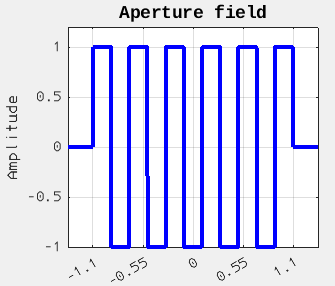
\includegraphics[width=125px]{aperture_ex.png}
    \end{center}
    \caption{Ejemplo de apertura tipo "grating" de longitud \qty{22}{\micro\meter}}
    \label{fig:aperture_ex}
\end{marginfigure}

\begin{align}
    k\sin\theta_x \pm k_0 = 0 \\
    \theta_x = \arcsin{\left(\frac{k_0}{k}\right)} \\
    \left\{
        \begin{aligned}
            \quad k &= \frac{2\pi}{\lambda} \quad \\
            k_0 &= \frac{2\pi N}{L}
        \end{aligned}
    \right\} \\
    \theta_x = \arcsin{\left(\frac{\lambda N}{L}\right)}
\end{align}

Donde $N$ tiene que ver con el numero de ranuras y es \num{5.5} en este caso\sidenote{Se ha escogido así para calcular la frecuencia del coseno enventanado. En el programa de simulación cuando se selecciona el máximo numero de ranuras se enventana una señal cuadrada de $N=\num{5.5}$ periodos. Vease la figura \ref{fig:aperture_ex}}. Los cálculos coinciden con las medidas de la simulación.

\newpage

\newthought{6. Evolución de la densidad de potencia con la distancia}

«Se trata de ver cómo evoluciona la potencia medida por un detector muy pequeño a medida que nos alejamos de la apertura (en el caso 2D).»

\begin{figure}[h]
    \begin{center}
        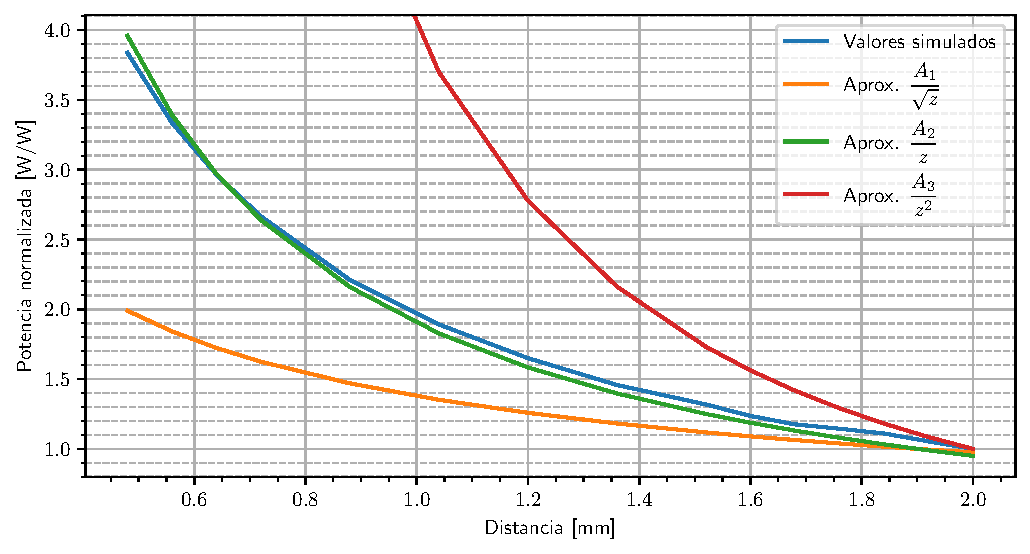
\includegraphics[width=300px]{p6.pdf}
    \end{center}
    \caption{Potencia normalizada segun la unidad en función de distancia de la apertura}
    \label{fig:p6}
\end{figure}

Tal y como en los cálculos teóricos, se puede observar que la potencia decae proporcionalmente a la inversa de la distancia. Por este motivo la aproximación que mas se acerca a los valores simulados (traza azul) es la traza verde $\frac{A_2}{z}$.

\end{document}
